%%%%%%%%%%%%%%%%%%%%%%%%%%%%%%%%%%%%%%%%%%%%%%%%%%%%%%%%%%%%%%%%%%%%%%%%%%%%%%%%
%2345678901234567890123456789012345678901234567890123456789012345678901234567890
%        1         2         3         4         5         6         7         8
%\documentclass[letterpaper, 10 pt, conference]{ieeeconf}  % Comment this line out if you need a4paper

\documentclass[a4paper, 11pt, conference]{ieeeconf}      % Use this line for a4 paper
\usepackage{amssymb}
\usepackage{graphicx} 
\usepackage{url} 

\IEEEoverridecommandlockouts                              % This command is only needed if 
                                                          % you want to use the \thanks command

\overrideIEEEmargins                                      % Needed to meet printer requirements.


\addtolength{\topskip}{-10pt}  % Adjust the value to fine-tune
\addtolength{\textheight}{10pt} % Ensure content fits in the original page area
\addtolength{\topmargin}{-10pt} % Reduce top margin

%In case you encounter the following error:
%Error 1010 The PDF file may be corrupt (unable to open PDF file) OR
%Error 1000 An error occurred while parsing a contents stream. Unable to analyze the PDF file.
%This is a known problem with pdfLaTeX conversion filter. The file cannot be opened with acrobat reader
%Please use one of the alternatives below to circumvent this error by uncommenting one or the other
%\pdfobjcompresslevel=0
%\pdfminorversion=4

% See the \addtolength command later in the file to balance the column lengths
% on the last page of the document

% The following packages can be found on http:\\www.ctan.org
%\usepackage{graphics} % for pdf, bitmapped graphics files
%\usepackage{epsfig} % for postscript graphics files
%\usepackage{mathptmx} % assumes new font selection scheme installed
%\usepackage{times} % assumes new font selection scheme installed
%\usepackage{amsmath} % assumes amsmath package installed
%\usepackage{amssymb}  % assumes amsmath package installed

\title{\vspace{-25pt}\LARGE \bf
Motion Planning for Indoor Fire Fighter Drone
}


\author{O. Devos 5245982 \\ C. Espirito Santo 5557917 \\ L. Le Ba 6291325 \\ N. Nanvani 6140289}%



\begin{document}



\maketitle
\thispagestyle{empty}
\pagestyle{empty}


%%%%%%%%%%%%%%%%%%%%%%%%%%%%%%%%%%%%%%%%%%%%%%%%%%%%%%%%%%%%%%%%%%%%%%%%%%%%%%%%
\begin{abstract}

This project develops a quadrotor drone system for emergency response in hazardous indoor environments. Using A*, RRT*, and motion primitives for motion planning, combined with PID and LQR controllers, the drone navigates efficiently to target locations. Simulations in PyBullet evaluate performance based on path length, solving time, and obstacle clearance, aiming to improve drone reliability in emergencies.

\end{abstract}

%%%%%%%%%%%%%%%%%%%%%%%%%%%%%%%%%%%%%%%%%%%%%%%%%%%%%%%%%%%%%%%%%%%%%%%%%%%%%%%%
\section{INTRODUCTION}
Quadrotor drones have become indispensable in emergency scenarios such as fires, gas leaks, and floods, offering a safer alternative to human intervention in hazardous environments. Their ability to navigate confined spaces and perform critical tasks makes them ideal for indoor applications, such as reaching danger zones or delivering fire-suppressing agents.

This project aims to develop a quadrotor drone system capable of navigating complex indoor spaces efficiently. To achieve this, motion planning algorithms like A*, RRT*, and motion primitives are explored, paired with PID and LQR controllers for accurate trajectory tracking. Simplifications, such as assuming a known static environment and modeling obstacles as convex shapes with safety buffers, ensure computational efficiency while maintaining reliability.

Simulations in PyBullet are used to evaluate the system in randomized building layouts, focusing on metrics such as path length, solving time, and obstacle clearance. This approach aims to enhance drone capabilities for safer and more effective emergency response operations.

\section{Problem Definition}
The selected real-world scenario involves the use of drones in emergency situations within buildings or building complexes, where drones can reduce the need for human intervention. Such applications are particularly relevant in scenarios like fires, gas leaks, or flooding, where human presence poses significant danger. Consequently, the robot morphology chosen for control is a quadrotor. The purpose of this quadrotor is to navigate from a starting point (e.g., a docking station) to a goal (e.g., the location of a fire inside a building), where it performs a designated task (e.g., extinguishing the fire by deploying water or a fire extinguisher bomb).

\begin{figure}[!h]
    \centering
    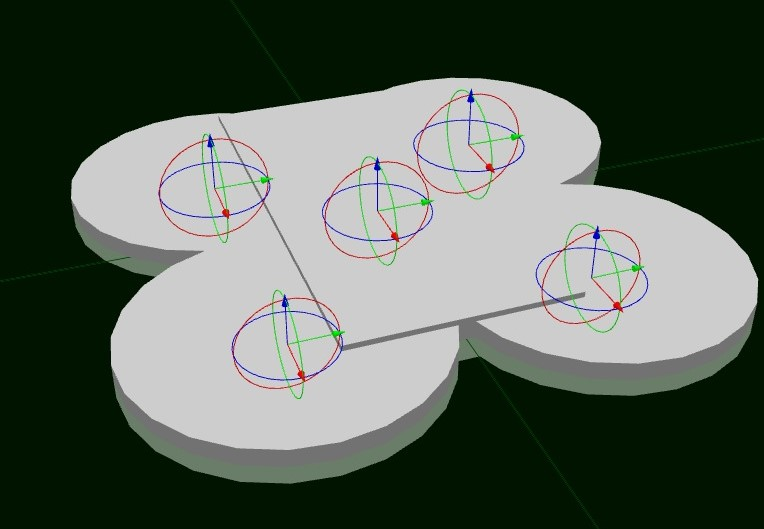
\includegraphics[width=0.4\textwidth]{drone_urdf_mockup.jpg}
    \caption{URDF visualization of our drone \cite{mmyself_ros_ardrone}}
    \label{fig:URDF}
\end{figure}

\section{Drone Modeling and Assumptions}
To visualize the quadrotor in the later stages within the simulation environment, the model from \texttt{gym-pybullet-drones} is employed. The propellers and aircraft are assumed to be a rigid body, and the quadrotor frame is symmetrical (as shown in Figure \ref{fig:URDF}). Taking into account the model’s given characteristics, as well as the well-established kinematics of a quadrotor, the following equations of motion are formulated under the assumption of keeping the drone flat:

\begin{figure}[!h]
    \centering
    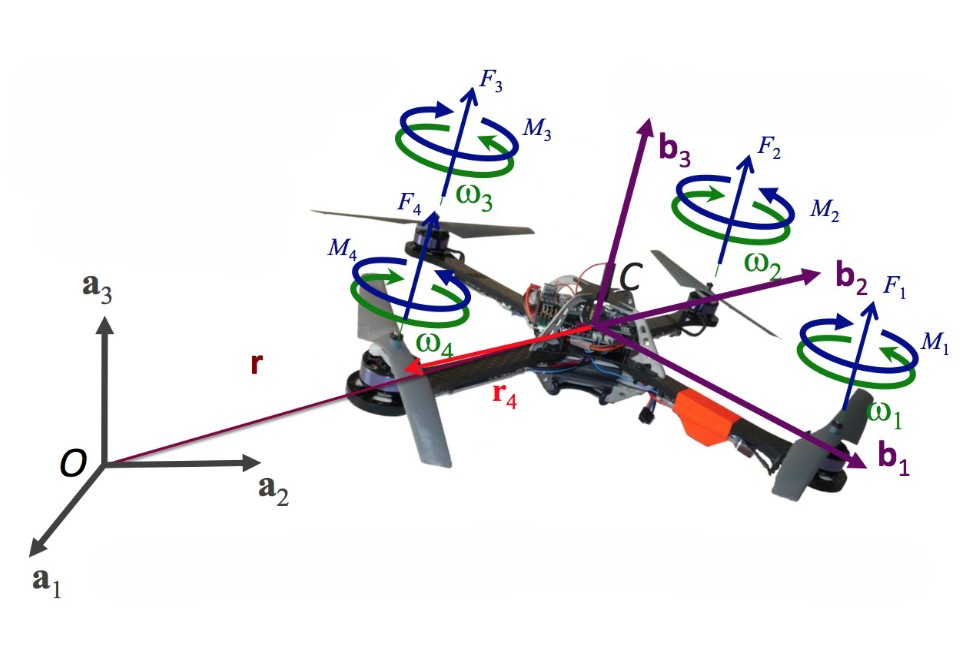
\includegraphics[width=0.4\textwidth]{mav_model.jpg}
    \caption{FBD of a simplified quadrotor \cite{MAV_Modeling_Control}}
    \label{fig:FBD}
\end{figure}

\begin{equation}
    F_i = k_T \rho D^4 \omega_i^2
    \label{eq:Forces}
\end{equation}
\begin{equation}
    M_i = k_Q \rho D^5 \omega_i^2
    \label{eq:Torques}
\end{equation}

\noindent For these, the variables are defined as:
\begin{itemize}
    \item $F_i$: Thrust force generated per $i$-th propeller \\ $i \in \{1,2,3,4 \}$, $N$.
    \item $M_i$: Torque generated per $i$-th propeller, $Nm$.
    \item $\omega_i$: Angular velocity per $i$-th propeller, $rad/s$.
    \item $k_T$: Thrust Coefficient based on propeller design.
    \item $k_Q$: Torque Coefficient based on propeller design.
    \item $\rho$: Air density.
    \item $D$: Propeller diameter.
\end{itemize}

Figure \ref{fig:FBD} shows the free-body diagram of the used quadrotor and therefore visualizes the acting forces and torques which are expressed in Eq. (\ref{eq:Forces}) and (\ref{eq:Torques}).

\section{Motion Planning and Configuration Space}
These equations are essential for the controller to follow the path generated by the motion planning algorithm. The motion planning algorithm plans an optimal trajectory for the robot to reach its goal via the most efficient path. In the given use case, the optimal path corresponds to the trajectory that minimizes the time required to reach the goal.

The configuration space of a quadrotor is $SE(3)$, which can be reduced to $\mathbb{R}^3 \times S^1$ via differential flatness. Here, $\mathbb{R}^3$ represents the translational position $(x,y,z)$ and $S^1$ represents the yaw orientation $\Psi$. Differential flatness allows simplification of the configuration space by deriving the remaining variables, roll $\phi$ and pitch $\theta$, from the position and yaw. Thus, the quadrotor is controlled by four independent inputs from its propellers. 

\section{Path Planning Approaches}
Based on the assumptions of the project, we assume a fully known static map, without incorporating real-time sensor data into the planning process. The robot is treated as holonomic, and a holonomic path planning approach is chosen. To select the most suitable route, three different path planners will be explored and compared:

\begin{enumerate}
    \item \textbf{A* Algorithm:} A graph-based planner known for its speed and optimal nature.
    \item \textbf{RRT*:} A sampling-based method effective for handling high-dimensional spaces efficiently and optimally.
    \item \textbf{Motion Primitives:} A combined approach using precomputed motion primitives for generating feasible trajectories.
\end{enumerate}

\section{Control Strategies}
Compatible controllers are essential for each planning approach:
\begin{itemize}
    \item \textbf{A*:} The planner generates a discrete set of waypoints that are smoothed before tracking. A PID controller is used due to its simplicity and low computational intensity.
    \item \textbf{RRT*:} A feedforward-feedback controller such as LQR is applied to efficiently track paths in real-time.
    \item \textbf{Motion Primitives:} LQR is also used for tracking the dynamically feasible trajectories produced by motion primitives.
\end{itemize}

\section{Obstacle Representation and Simplification}
To ensure effective trajectory planning, the obstacles within the environment are appropriately constrained and represented. Structural walls are considered fixed obstacles, while furniture and other items are overestimated as simple rectangular convex shapes. This simplification reduces computational complexity and facilitates node and vertex generation for motion planning algorithms. A buffer zone is added around obstacles to enhance safety and reliability.

\section{Performance Evaluation}
A custom loss function will be developed to validate performance. This function includes:
\begin{itemize}
    \item Solving time (path generation).
    \item Execution time (time required for simulation).
    \item Path length.
    \item Weighted average distance from the closest obstacle at each timestep.
\end{itemize}
Recording these metrics provides a quantifiable basis for evaluating the effectiveness of different approaches.

\section{Simulation Environment}
The robot operates in a simulated environment consisting of multiple buildings with various floor plans. The task involves flying to a designated emergency location. The assumptions include open doors and windows to avoid additional complexity. The environment will be randomized for evaluation. The PyBullet library will facilitate physics simulation and visualization.

%\addtolength{\textheight}{-12cm}   % This command serves to balance the column lengths
                                  % on the last page of the document manually. It shortens
                                  % the textheight of the last page by a suitable amount.
                                  % This command does not take effect until the next page
                                  % so it should come on the page before the last. Make
                                  % sure that you do not shorten the textheight too much.

%%%%%%%%%%%%%%%%%%%%%%%%%%%%%%%%%%%%%%%%%%%%%%%%%%%%%%%%%%%%%%%%%%%%%%%%%%%%%%%%



%%%%%%%%%%%%%%%%%%%%%%%%%%%%%%%%%%%%%%%%%%%%%%%%%%%%%%%%%%%%%%%%%%%%%%%%%%%%%%%%



%%%%%%%%%%%%%%%%%%%%%%%%%%%%%%%%%%%%%%%%%%%%%%%%%%%%%%%%%%%%%%%%%%%%%%%%%%%%%%%%



\bibliographystyle{plain} 
\bibliography{refs}

\end{document}
